\documentclass[xcolor=dvipsnames]{beamer}
\useoutertheme{infolines}
\setbeamertemplate{navigation symbols}{}
\setbeamertemplate{items}[ball]
\usepackage{graphicx,multirow,color,xcolor,verbatim,float,comment,amsmath}
\setbeamertemplate{frametitle}[default][center]
\begin{document}
\title{Validation of MVGA by a toy example}
\author{Bowen Deng}
\institute{Dept. of Prob. and Stat.}
\date{}
\begin{frame}
\maketitle
\end{frame}
\begin{frame}
\tableofcontents
\end{frame}
\section{Review}
\begin{frame}{MVGA}
We could generalize the GA algorithm to multiple value case.\\
Most steps are similar, but the crossproduction is much harder.\\
Let $k_{\min}=k_{\max}=2$,\\
Father:\\
11223300\\
Mother:\\
22331100\\
Their child should inherit two 1s, two 2s and two 3s. But the child should be as distinct from its parents as possible.\\
\end{frame}
\begin{frame}{Crossproduct}
Denote father: $F=(a_1,\cdots,a_n)$, mother: $M=(b_1,\cdots,b_n)$, $a_i,b_i\in\{0,1,\cdots,t\}$.\\
$a_i=\rho$ means i-th gene is in the $\rho$-th set, if $\rho=0$, i-th gene is not selected.\\
The motivation is to find a feasible solution corresponding to child $c_1,\cdots,c_n$ under constraint:\\
\[
\sum_{i=1}^n[(1-x_i)\mathrm{I}(a_i=\rho)+x_i\mathrm{I}(b_i=\rho)]\in[k_{\min},k_{\max}]
\]
where $x_i=0$ represents $c_i=a_i$, and $x_i=1$ represents $c_i=b_i$.\\
Moreover,\\
\[\sum_{a_i\text{ or }b_i>0}x_i\in[\frac{s-c}{2},\frac{s+c}{2}].\]
where $s=\#\{a_i\text{ or }b_i>0\}$.\\
We should minimize $c$ (ILP).\\
\end{frame}
\begin{frame}{Discussion}
At first glance, we plug an ILP inside of a genetic algorithm, the computation is expensive.\\
However, we only need to involve $|F\cup M|\leqslant 2tk_{\max}\ll n$ binary variables and one integer variable.\\
\end{frame}
\section{Toy Example}
\begin{frame}
We consider the hidden set detection problem:\\
Suppose there are $S_1,\cdots,S_t\subset \{1,\cdots,n\}$, we would like to detect those sets without prior knowledge.\\
We could use a test set $M$ and get its matching score with those hidden sets. For convenience, let $S(M)=n-\min_{1\leqslant\rho\leqslant t} |M\triangle S_{\rho}|$.\\
An iterative detection is to find maximizer $\hat{M}=\arg\max S(M)$, deleting $\hat{M}$, repeat.\\
The simultaneous version would be $\max(M_1,\cdots,M_t)=\sum_{i=1}^t S(M_i)$.\\
\end{frame}
\begin{frame}
This problem is similar to our task, and we use this toy problem to test the methods.\\
We use MVGA to test whether it converges in this problem.\\
For the sake of computation cost, we let $S_1=\{1,\cdots,5\}, S_2=\{6,\cdots,10\}$, $n=20$. And we find $M_1$, $M_2$ simultaneously using MVGA.\\
\begin{table}
\begin{tabular}{cccc}
\hline
Population&Iteration&Score&Time(s)\\
\hline
\multirow{3}{*}{100}&1&34&52\\
&10&37&135.41\\
&20&39&206.07\\
\multirow{3}{*}{10}&1&32&12\\
&10&34&10.19\\
&20&33&44.97\\
50&20&38&115.43\\
\end{tabular}
\end{table}
\end{frame}
\section{Parameter Selection on Original Problem}
\begin{frame}
We use permutation test to identify the best $t$.\\
For simulation data with $t=2$.\\
\begin{figure}
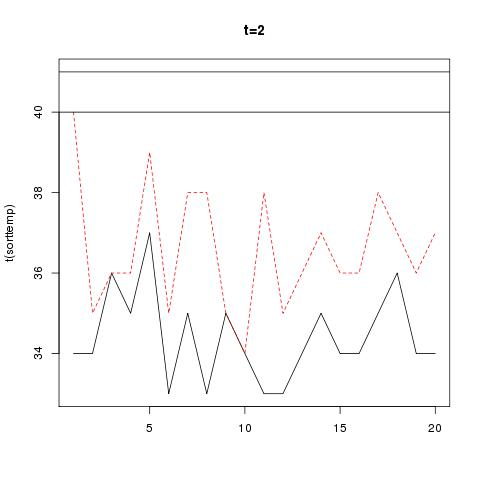
\includegraphics[width=0.8\linewidth]{figure2.png}
\end{figure}\end{frame}
\begin{frame}\begin{figure}
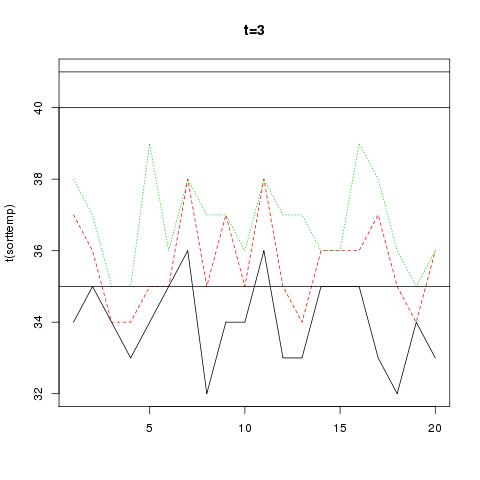
\includegraphics[width=0.8\linewidth]{figure3.png}
\end{figure}\end{frame}
\begin{frame}\begin{figure}
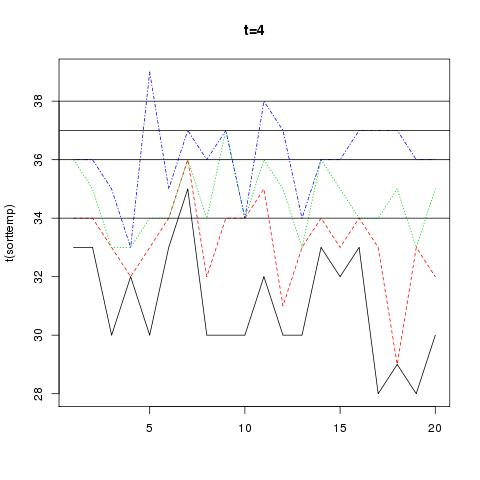
\includegraphics[width=0.8\linewidth]{figure4.png}
\end{figure}\end{frame}
\begin{frame}
loose to $0\leqslant x\leqslant 1$.\\
$u=f(u)$\\
lars
\end{frame}
\end{document}
